
It is desirable that numerous commercial robot systems be able to 
immediately execute the plan for the series of actions required to transition from the initial state
to the goal state of the kitting problem. However, there is currently no
accepted standard robot programming language. For this reason, the authors
have developed a canonical robot control language that attempts to be
a lowest common denominator of robot programing languages. It is anticipated
that kitting plans can be translated into  CRCL command sets which may then be
evaluated by standardized metric software. The CRCL command sets may then
be translated into a specific robot platform's language.

The syntax of commands is given below using C++ syntax. The command
name is given followed by the command arguments (if any) in parentheses,
including the types of the arguments.
Note that the robot cannot be commanded by canonical robot commands in
terms of its joint angles (or distances).

Three of the CRCL commands use the Pose structure. The Pose structure gives
the location and orientation of the coordinate system of the controlled
object in the units of the current operating coordinate system. 
The controlled object is the gripper if the robot has one attached
or the outermost component of the robot arm if not.  The location is
specified by the point in current operating coordinates at which the
origin of the coordinate system of the controlled object lies. The point is
described by giving its X, Y, and Z values. The orientation of the
controlled object is specified by giving the I, J, and K components in
current operating coordinates of the Z and X axes of the coordinate
system of the controlled object. 

The complete list of CRCL commands follows.

\begin{itemize}

\item \sf CloseGripper() \rm -- close the gripper.\\

\item \sf CloseToolChanger() \rm -- close the tool changer on the robot so
  that it attaches to a tool. The robot must be in an appropriate position
  with respect to the tool for the changer mechanism on the robot to attach
  to the tool.\\

\item \sf Dwell (double time) \rm -- stay motionless for the given amount
  of \sf time \rm in seconds.\\

\item \sf EndCanon(int reason) \rm -- do whatever is necessary to stop
  executing canonical robot commands. No specific action is required. The
  robot controller should not execute any canonical robot command except
  \sf InitCanon \rm after executing \sf EndCanon \rm and should signal an
  error if it is given one.  This command will normally be given when
  execution of a plan is complete.  It may also be given if the plan
  interpreter detects an error in the plan or is unable to proceed for any
  other reason. A value of 0 for \sf reason \rm indicates that execution of
  a plan has completed successfully.  A positive value of reason indicates
  not.\\

\item \sf InitCanon() \rm -- do whatever is necessary to get ready to
move. Length units, angle units, and operating coordinate system are 
set to the default units. This command
will normally be given when the plan interpreter opens a plan to be
executed.\\

\item \sf Message (string message) \rm -- display the given \sf message \rm
  on the operator console.\\

\item \sf MoveStraightTo(Pose * pose) \rm -- move the controlled point in a
  straight line from the current pose to the given \sf pose\rm, and stop
  there.\\

\item \sf MoveThroughTo(Pose ** poses, int numPoses) \rm -- move the
  controlled point along a trajectory passing near all but the last of the
  given \sf poses\rm, and stop at the last of the given \sf poses\rm.
  The \sf numPoses \rm gives the number of poses.\\

\item \sf MoveTo(Pose * pose) \rm -- move the controlled point along any
  convenient trajectory from the current pose to the given \sf pose\rm,
  and stop there.\\

\item \sf OpenGripper() \rm -- open the gripper.\\

\item \sf OpenToolChanger() \rm -- open the tool changer on the robot so
  that it releases the end effector.  This is normally done after the end
  effector attached to the robot has been moved into an end effector
  changer.\\

\item \sf SetAbsoluteAcceleration(double acceleration) \rm -- set the
  acceleration for the controlled point to the given value in length units
  per second per second.\\

\item \sf SetAbsoluteSpeed(double speed) \rm -- set the speed for the
  controlled point to the given value in length units per second.\\

\item \sf SetAngleUnits(string UnitName) \rm -- set angle units to the unit
  named by the \sf UnitName\rm.  The \sf UnitName \rm must be one of
  ``degree'' or ``radian''. All commands that use angle units (for
  orientation or orientation tolerance) are in terms of those angle
  units. Existing values for orientation are converted automatically to the
  equivalent value in new angle units.  The default angle unit is
  ``degree''.\\

\item \sf SetCoordinateFrame(string CoordSystem) \rm -- set the
operating coordinate system to the system referred to by
\sf CoordSystem\rm. The \sf CoordSystem \rm must be one of
``Workstation", ``RobotBase", or ``ToolTip".\\

\item \sf SetEndAngleTolerance(double tolerance) \rm -- set the tolerance
  for the orientation of the end of the arm (whenever there is no gripper
  there) or of the gripper (whenever a gripper is on the end of the arm) to
  the given value in current angle units. This applies to the X-axis direction
and the Z-axis direction.\\

\item \sf SetEndPointTolerance(double tolerance) \rm -- set the tolerance
  for the position of the end of the arm (whenever there is no gripper
  there) or of the tool centre point (whenever a gripper is on the end of
  the arm) to the given value in current length units.\\

\item \sf SetIntermediatePointTolerance(double tolerance) \rm -- set the
  tolerance for smooth motion near intermediate points to the given value
  in current length units.\\

\item \sf SetLengthUnits(string UnitName) \rm -- set length units to the
  unit named by the \sf UnitName\rm.  The \sf UnitName \rm must be one of
  ``inch'', ``mm'' or ``meter''. All commands that use length units (for
  location, tolerance, speed, and acceleration) are in terms of those
  length units. Existing values for speed, position, acceleration, etc. are
  converted automatically to the equivalent value in new length units. The
  default length unit is millimeters, ``mm''.\\

\item \sf SetRelativeAcceleration(double percent) \rm -- set the
  acceleration for the controlled point to the given percentage of the
  robot's maximum acceleration.\\

\item \sf SetRelativeSpeed(double percent) \rm -- set the speed for the
  controlled point to the given percentage of the robot's maximum speed.\\

%\vspace{.1in} \sf The next two items do not seem to really belong here. I understand why
%Teddy put them here (he needed the commands), but they seem too specific.
%Any suggestions on how to make them more general? I was thinking of a
%general ``StartRobotSubSystem(string name, string parameter)". \rm \\ \\
%\item \sf StartObjectScan(string name) \rm -- Activate the object sensor,
%  if it isn't already activated, and add the given \sf name \rm to the list of
%  parts being searched for.\\
%
%\item \sf StopObjectScan() \rm -- deactivate the object sensor.\\

\item \sf StopMotion(integer isEmergency) \rm -- stop the robot motion. If
  \sf isEmergency \rm is not 0, then stop as soon as possible regardless of
  damage to the system. If \sf isEmergency \rm is 0 then come to a graceful
  stop.\\

\end{itemize}

\begin{flushleft}
	\begin{figure}[ht]
		\fbox{
			\begin{minipage}{3.2in}
				\sf
				\begin{tabbing}
					xxx\=xx\=xx\=\kill
					InitCanon()\\	
					SetLengthUnits("meter")\\
					CloseGripper()\\
					CloseToolChanger()\\
					Dwell(1.7)\\
					Message("This message is false")\\
					SetRelativeSpeed(50.0)\\
					SetAbsoluteSpeed(3.8)\\
					MoveThroughTo(\{\{\{5,0,2\}, \{0,0,1\}, \{1,0,0\}\},\\
					\>\{\{5,8,2\}, \{0,0,1\}, \{1,0,0\}\},\\
					\>\{\{7,8,2\}, \{0,0,1\}, \{1,0,0\}\}\}, 3)\\
					MoveStraightTo(\{\{4,8,2\}, \{0,0,1\}, \{1,0,0\}\})\\
					MoveTo(\{\{9,8,2\}, \{0,0,1\}, \{1,0,0\}\})\\
					OpenGripper()\\
					OpenToolChanger()\\
					SetAbsoluteAcceleration(0.95)\\
					SetAngleUnits("degree")\\
					SetEndAngleTolerance(1.3)\\
					SetEndPointTolerance(0.4)\\
					SetIntermediatePointTolerance(10.734)\\
					SetLengthUnits("mm")\\
					SetRelativeAcceleration(0.8)\\
					SetRelativeSpeed(0.75)\\
					SetRelativeAcceleration(-110)\\
					MoveStraightTo(87)\\
					EndCanon(2)\\
				\end{tabbing}
				\rm
			\end{minipage}
		}
		\caption{Kitting Plan for Testing}
		\label{fig:KittingPlan}
	\end{figure}
\end{flushleft}

A file format for representing CRCL commands has been devised.
Figure~\ref{fig:KittingPlan} shows an example of a file prepared using this
format. A C++ class model of CRCL commands has been built, and a parser has
been built in C++ for reading CRCL files and populating
CRCL class instances.

\subsection{Plan Model}
The kitting system presented in this document relies on a \textit{direct} model of execution where the executor directly performs the activities specified in the plan. Figure~\ref{fig:executor} depicts the executor process for the kitting domain where ellipses represent files, regular rectangles are used to define processes, and rounded rectangles illustrate tools. The red dashed box contains the processes part of the executor. The components in Figure~\ref{fig:executor} are described below:

\begin{enumerate}
\item PDDL domain and problem files are currently generated by hand from the IEEE RAS  Ontologies for Robotics and Automation Working Group's
OWL-based knowledge representation
and are used by an open source planner from Coles et al. \cite{Coles.ICAPS.2010} to automatically generate a plan file. In the near future, these files will be automatically generated.
The plan file contains a sequence of actions that can be executed from the initial state and that lead to a goal state. The actions present in the plan file are originally defined in the PDDL domain file. The initial and goal states are defined in the PDDL problem file.

\item The interpreter takes the plan file as input and builds the corresponding CRCL file. Real time information on the environment is required in order to fill in information required by the CRCL on
object locations. Since both the OWL and XML implementations of the knowledge representation are file based, real time information proved to be problematic. In order to solve this problem,
an automatically generated MySQL database \cite{MySQL} has been introduced as part of the knowledge representation. More details on this database are provided in Section \ref{sect:MySQL}.
Table~\ref{tab:takepart} shows an example of CRCL commands generated for the PDDL action \stvar{take-part(part\_b\_1)}. Please note that the PDDL action \stvar{take-part} developed for the current kitting domain has more than one parameter. Not all the parameters are relevant for the example depicted in Table~\ref{tab:takepart} and the number of parameters has been  reduced for simplicity. In this example,
the locations of the \lq\lq{}MoveTo\rq\rq{} commands would come from the MySQL database.

\begin{table}[h!]
\centering

    \begin{tabular}{l}
    \stvar{take-part(part\_b\_1)}\\
    \hline
    \hline
  \texttt{\scriptsize{Message (``take part part\_b\_1")}}\\
  \texttt{\scriptsize{MoveTo(\{\{-0.03, 1.62, -0.25\}, \{0, 0, 1\}, \{1, 0, 0\}\})}}\\
  \texttt{\scriptsize{Dwell (0.05)}}\\
  \texttt{\scriptsize{MoveTo(\{\{-0.03, 1.62, 0.1325\}, \{0, 0, 1\}, \{1, 0, 0\}\})}} \\
  \texttt{\scriptsize{CloseGripper ()}} \\
  \texttt{\scriptsize{MoveTo(\{\{-0.03, 1.62, -0.25\}, \{0, 0, 1\}, \{1, 0, 0\}\})}}\\
  \texttt{\scriptsize{Dwell (0.05)}}\\
  \hline
  \end{tabular}
\caption{An example of CRCL commands for a PDDL action}
  \label{tab:takepart}
\end{table}

\item The CRCL file is used by the controller to create ROS commands.

\item The ROS commands are used by the ROS software controller for a robotic arm to initiate actual execution of actions.

\end{enumerate}

\begin{figure}[ht!]
\begin{center}
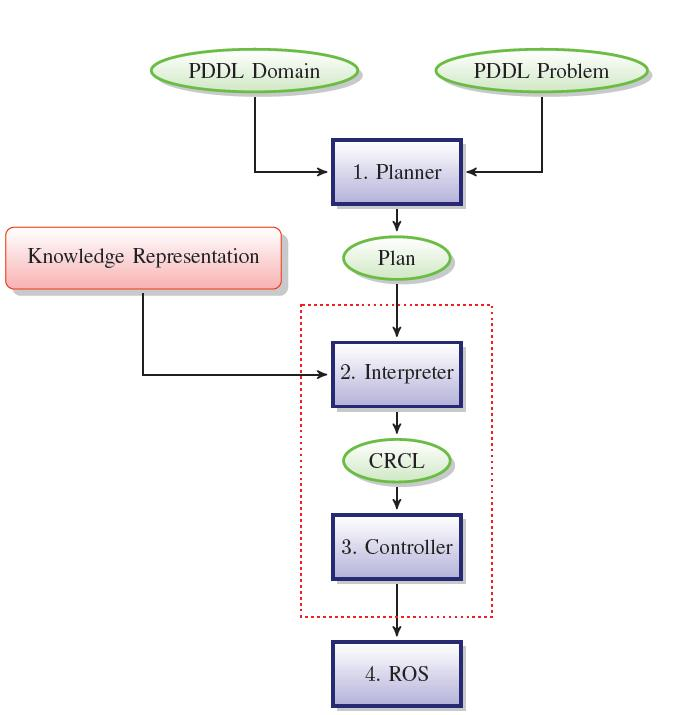
\includegraphics[width=8cm]{images/executordiag.jpg}
\caption{The executor process}
\label{fig:executor}
\end{center}
\end{figure}

